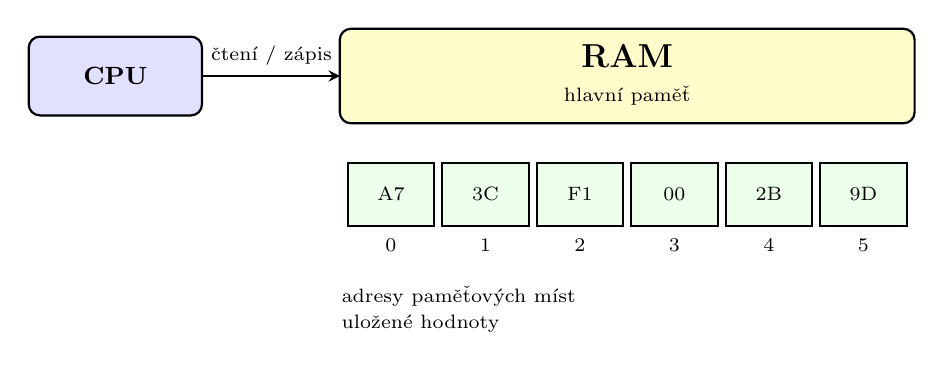
\begin{tikzpicture}[
    x=1cm, y=1cm,
    >=stealth,
    every node/.style={font=\small},
    box/.style={
        draw,
        thick,
        rounded corners,
        align=center
    },
    cell/.style={
        draw,
        thick,
        minimum width=1.1cm,
        minimum height=0.8cm,
        align=center,
        fill=green!8
    },
    arr/.style={->, thick}
]

    % CPU
    \node[
        box,
        fill=blue!12,
        minimum width=2.2cm,
        minimum height=1.0cm
    ] (cpu) at (-5.5,0.8) {\textbf{CPU}};

    % RAM title
    \node[
        box,
        fill=yellow!20,
        minimum width=7.3cm,
        minimum height=1.2cm
    ] (rambox) at (1.0,0.8) {};

    \node[font=\bfseries\large] at (1.0,1.05) {RAM};
    \node[font=\scriptsize] at (1.0,0.55) {hlavní paměť};

    % Arrow CPU -> RAM
    \draw[arr] (cpu.east) -- node[above, font=\scriptsize] {čtení / zápis} (-2.65,0.8);

    % Linear memory cells
    \node[cell] (c0) at (-2.0,-0.7) {};
    \node[cell] (c1) at (-0.8,-0.7) {};
    \node[cell] (c2) at (0.4,-0.7) {};
    \node[cell] (c3) at (1.6,-0.7) {};
    \node[cell] (c4) at (2.8,-0.7) {};
    \node[cell] (c5) at (4.0,-0.7) {};

    % Cell values
    \node[font=\scriptsize] at (-2.0,-0.7) {A7};
    \node[font=\scriptsize] at (-0.8,-0.7) {3C};
    \node[font=\scriptsize] at (0.4,-0.7) {F1};
    \node[font=\scriptsize] at (1.6,-0.7) {00};
    \node[font=\scriptsize] at (2.8,-0.7) {2B};
    \node[font=\scriptsize] at (4.0,-0.7) {9D};

    % Addresses
    \node[font=\scriptsize] at (-2.0,-1.35) {0};
    \node[font=\scriptsize] at (-0.8,-1.35) {1};
    \node[font=\scriptsize] at (0.4,-1.35) {2};
    \node[font=\scriptsize] at (1.6,-1.35) {3};
    \node[font=\scriptsize] at (2.8,-1.35) {4};
    \node[font=\scriptsize] at (4.0,-1.35) {5};

    % Labels
    \node[anchor=west, font=\scriptsize] at (-2.75,-2.0) {adresy paměťových míst};
    \node[anchor=west, font=\scriptsize] at (-2.75,-2.35) {uložené hodnoty};

\end{tikzpicture}
